\documentclass[10pt]{article}
\setlength{\oddsidemargin}{0.25 in}
\setlength{\evensidemargin}{-0.25 in}
\setlength{\topmargin}{-0.6 in}
\setlength{\textwidth}{6.5 in}
\setlength{\textheight}{8.5 in}
\setlength{\headsep}{0.75 in}
\setlength{\parindent}{0 in}
\setlength{\parskip}{0.1 in}

\usepackage{graphicx}
\usepackage{url}

\usepackage{float}
\usepackage{hyperref}

%
% The following commands sets up the lecnum (lecture number)
% counter and make various numbering schemes work relative
% to the lecture number.
%
\newcounter{lecnum}
\renewcommand{\thepage}{\thelecnum-\arabic{page}}
\renewcommand{\thesection}{\thelecnum.\arabic{section}}
\renewcommand{\theequation}{\thelecnum.\arabic{equation}}
%\renewcommand{\thefigure}{\thelecnum.\arabic{figure}}
\renewcommand{\thetable}{\thelecnum.\arabic{table}}
\newcommand{\dnl}{\mbox{}\par}

%
% The following macro is used to generate the header.
%
\newcommand{\lecture}[4]{
  \pagestyle{myheadings}
  \thispagestyle{plain}
  \newpage
  \setcounter{lecnum}{#1}
  \setcounter{page}{1}
  \noindent
  \begin{center}
  \framebox{
     \vbox{\vspace{2mm}
   \hbox to 6.28in { {\bf CMPSCI~630~~~Systems
                       \hfill Spring 2023} }
      \vspace{4mm}
      \hbox to 6.28in { {\Large \hfill Lecture #1  \hfill} }
%       \hbox to 6.28in { {\Large \hfill Lecture #1: #2  \hfill} }
      \vspace{2mm}
      \hbox to 6.28in { {\it Lecturer: #3 \hfill Scribe: #4} }
     \vspace{2mm}}
  }
  \end{center}
  \markboth{Lecture #1: #2}{Lecture #1: #2}
  \vspace*{4mm}
}

%
% Convention for citations is authors' initials followed by the year.
% For example, to cite a paper by Leighton and Maggs you would type
% \cite{LM89}, and to cite a paper by Strassen you would type \cite{S69}.
% (To avoid bibliography problems, for now we redefine the \cite command.)
%
\renewcommand{\cite}[1]{[#1]}

% \input{epsf}

%Use this command for a figure; it puts a figure in wherever you want it.
%usage: \fig{NUMBER}{FIGURE-SIZE}{CAPTION}{FILENAME}
%\newcommand{\fig}[4]{
%           \vspace{0.2 in}
%           \setlength{\epsfxsize}{#2}
%           \centerline{\epsfbox{#4}}
%           \begin{center}
%           Figure \thelecnum.#1:~#3
%           \end{center}
%   }

% Use these for theorems, lemmas, proofs, etc.
\newtheorem{theorem}{Theorem}[lecnum]
\newtheorem{lemma}[theorem]{Lemma}
\newtheorem{proposition}[theorem]{Proposition}
\newtheorem{claim}[theorem]{Claim}
\newtheorem{corollary}[theorem]{Corollary}
\newtheorem{definition}[theorem]{Definition}
\newenvironment{proof}{{\bf Proof:}}{\hfill\rule{2mm}{2mm}}

% Some useful equation alignment commands, borrowed from TeX
\makeatletter
\def\eqalign#1{\,\vcenter{\openup\jot\m@th
 \ialign{\strut\hfil$\displaystyle{##}$&$\displaystyle{{}##}$\hfil
     \crcr#1\crcr}}\,}
\def\eqalignno#1{\displ@y \tabskip\@centering
 \halign to\displaywidth{\hfil$\displaystyle{##}$\tabskip\z@skip
   &$\displaystyle{{}##}$\hfil\tabskip\@centering
   &\llap{$##$}\tabskip\z@skip\crcr
   #1\crcr}}
\def\leqalignno#1{\displ@y \tabskip\@centering
 \halign to\displaywidth{\hfil$\displaystyle{##}$\tabskip\z@skip
   &$\displaystyle{{}##}$\hfil\tabskip\@centering
   &\kern-\displaywidth\rlap{$##$}\tabskip\displaywidth\crcr
   #1\crcr}}
\makeatother

% **** IF YOU WANT TO DEFINE ADDITIONAL MACROS FOR YOURSELF, PUT THEM HERE:



% Some general latex examples and examples making use of the
% macros follow.

\begin{document}

%FILL IN THE RIGHT INFO.
%\lecture{**LECTURE-NUMBER**}{**DATE**}{**LECTURER**}{**SCRIBE**}
\lecture{9}{March 21}{Emery Berger}{Sanath Upadhya}

\section{History of UNIX}

A brief history and impact of UNIX 
\begin{itemize}
  \item One of the most successful OS created
  \item UNIX inspired many of the current OS - foe example OSX, MINIX, Linux
  \item It was designed and developed by AT \& T Bell Labs (even C and C++ was developed by the same entity)
  \item Initially developed so that the developers could play video games and thus, UNIX was written so that it could be portable and run on different H/W platforms
  \item After UNIX became successful, AT \& T imposed a licensing fee. University of California Berkeley implemented the Application Binary Interface (ABI) to negate this and developed BSD having most of the functionality of UNIX.
  \item This ABI of BSD was then used by OSX, Windows etc.
  \item They also developed a kernel and its conceptual digram is as shown in the figure below

\begin{figure}[H]
\centering
\includegraphics[width=5cm, height=5cm]{concept.png}
\caption{Conceptual diagram of kernel \cite{\href{https://www.researchgate.net/figure/A-conceptual-diagram-of-a-Unix-system-The-kernel-surrounds-and-controls-the-hardware_fig5_2912001}{C1}}}
\label{fig:1}
\end{figure}
\item Kernel has access to everything and this runs in privileged mode
\item The user programs all run outside the kernel and the basic diagram of the user space and the kernel space is as shown in the figure below

\begin{figure}[H]
\centering
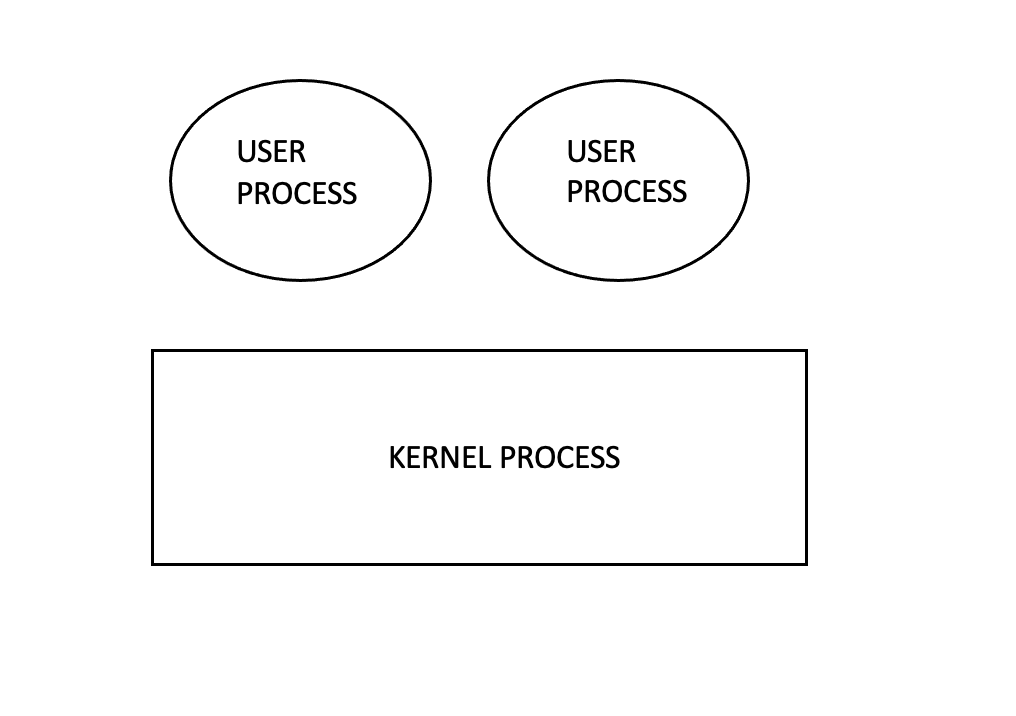
\includegraphics[width=4cm, height=4cm]{userkernel.png}
\caption{User space and kernel space}
\label{fig:2}
\end{figure}


\end{itemize}

\section{MULTICS}
\begin{itemize}
\item This OS was designed and developed by MIT, General Electric and Bell labs
\item Was written in a high level programming language PL/I
\item Was designed to run on multi core processors and was designed such that any processors could be removed while the OS was still running
\item As a result, it turned the OS problem into a distributed systems problem and thus was very complex
\item A lot of the features that was seen in UNIX was borrowed from MULTICS, and thus, UNIX was a limited version of MULTICS (UNIX was developed by former MULTICS programmers)

\end{itemize}


\section{Features borrowed from MULTICS}
\begin{itemize}
    \item Protected access and the privileges was borrowed from MULTICS
    \item Symbolic links
    \item Hierarchical file system
    \item Writing an OS in a high level language
    \item Security rings, i.e. privileged access (see conceptual diagram of kernel), with kernel being given the ring 0, ring 1 to the device drivers and ring 3 to the user applications. This privilege ring is baked into H/W
    \item Command line or shell was also borrowed from MULTICS
    
\end{itemize}

\section{Device drivers}
\begin{itemize}
    \item Device drivers usually reside in the kernel. These are the programs that directly interact with the H/W. 
    \item They offer some level of abstraction to the processes above that use these device drivers
    \item A device driver has to be written for every H/W and for every OS that supports this H/W (thus, an explosion of device drivers seen)
    \item To minimize this, the USB was created - one device driver that can handle multiple H/W devices. USBs have a DOS file system when you initially plug in
    \item Since the device drivers reside in kernel, a lot of security issues might be exposed if the device driver does not behave properly
    \item If a device driver overwrites memory in the kernel, we see kernel panic (and in Windows OS results in Windows Blue Screed of Death)
    \item To prevent this, MSFT had to do a lot of static checking of device driver code so that no untoward incidents happen
    \item They also decided to sign the device drivers, saying which are safe and which are not
    \item The fundamental question that arose out of this was whether the device drivers should reside in kernel or should be a part of the user space
    \item This lead to the development of micro-kernels, wherein only a small amount of functionality was kept in the kernel and everything else was moved out to the user space
    \item The corollary situation was the monolithic kernel, where all the functionality resided in the kernel itself

    \item Micro-kernel
    \begin{itemize}
        \item This was first instantiated by Any Tannebaum in MINIX (which is nothing but UNIX with a micro-kernel)
        \item Deployed on the H/W i386 (early version of x86 of Intel
        Thinking was, even if the device driver crashes, the overall system remains safe and one would just have to restart the device driver in such a scenario 
        \item However, the idea of micro-kernel did not take off due to performance issues
        \item We see that, every time there is transfer of control from user space to kernel space (i.e. context switching), there is a lot of copy operations performed (to save the state, get data from hard drive etc.). This is obviously much slower than a monolithic kernel, where this would just be a function call
        \item There is also the problem of caches being "warm" (i.e. all relevant data might already be in the cache), and when we do context switching, this all has to be flushed and has to be copied again, resulting in a performance hit
    \end{itemize}
    \item Thus, we see that monolithic kernels are the ones that are preferred in today's operating system
    \item Context switching is also used when different applications share the same CPU resource. This is also called as time slicing of programs
    \item Every program is allowed a certain quanta (one quanta is around 5ms, which is reasonably high), so that every program does some reasonable progress whenever it gets the CPU
    \item However, the idea of micro-kernel is still valid and this comes to TCB (trusted computing base)
    \item This means that find a small base where the trust resides (smaller the base, easier it is to analyse and detect security risks)
    \item Intel also has something like this called the SGX (secure enclaves) and they also have TEEC (trusted execution environments)
\end{itemize}

\section{UNIX file system}
\begin{itemize}
    \item UNIX took the concept of file abstraction (where everything is a file
    \item We also see that standard I/O are treated as files and < and > were introduced in UNIX
    \item Write to a file is a > foo.out
    \item Read from a file is a < in
    \item They also introduced the mounted file system which enabled the remote file system that we see today (like NFS)
    \item There is only one level of indirection - we can move the mounted file system anywhere to any directory in our local FS
    \item They also introduced the concept of i-nodes and direct/indirect addressing of files (as shown in figure below)
    \begin{figure}[H]
\centering
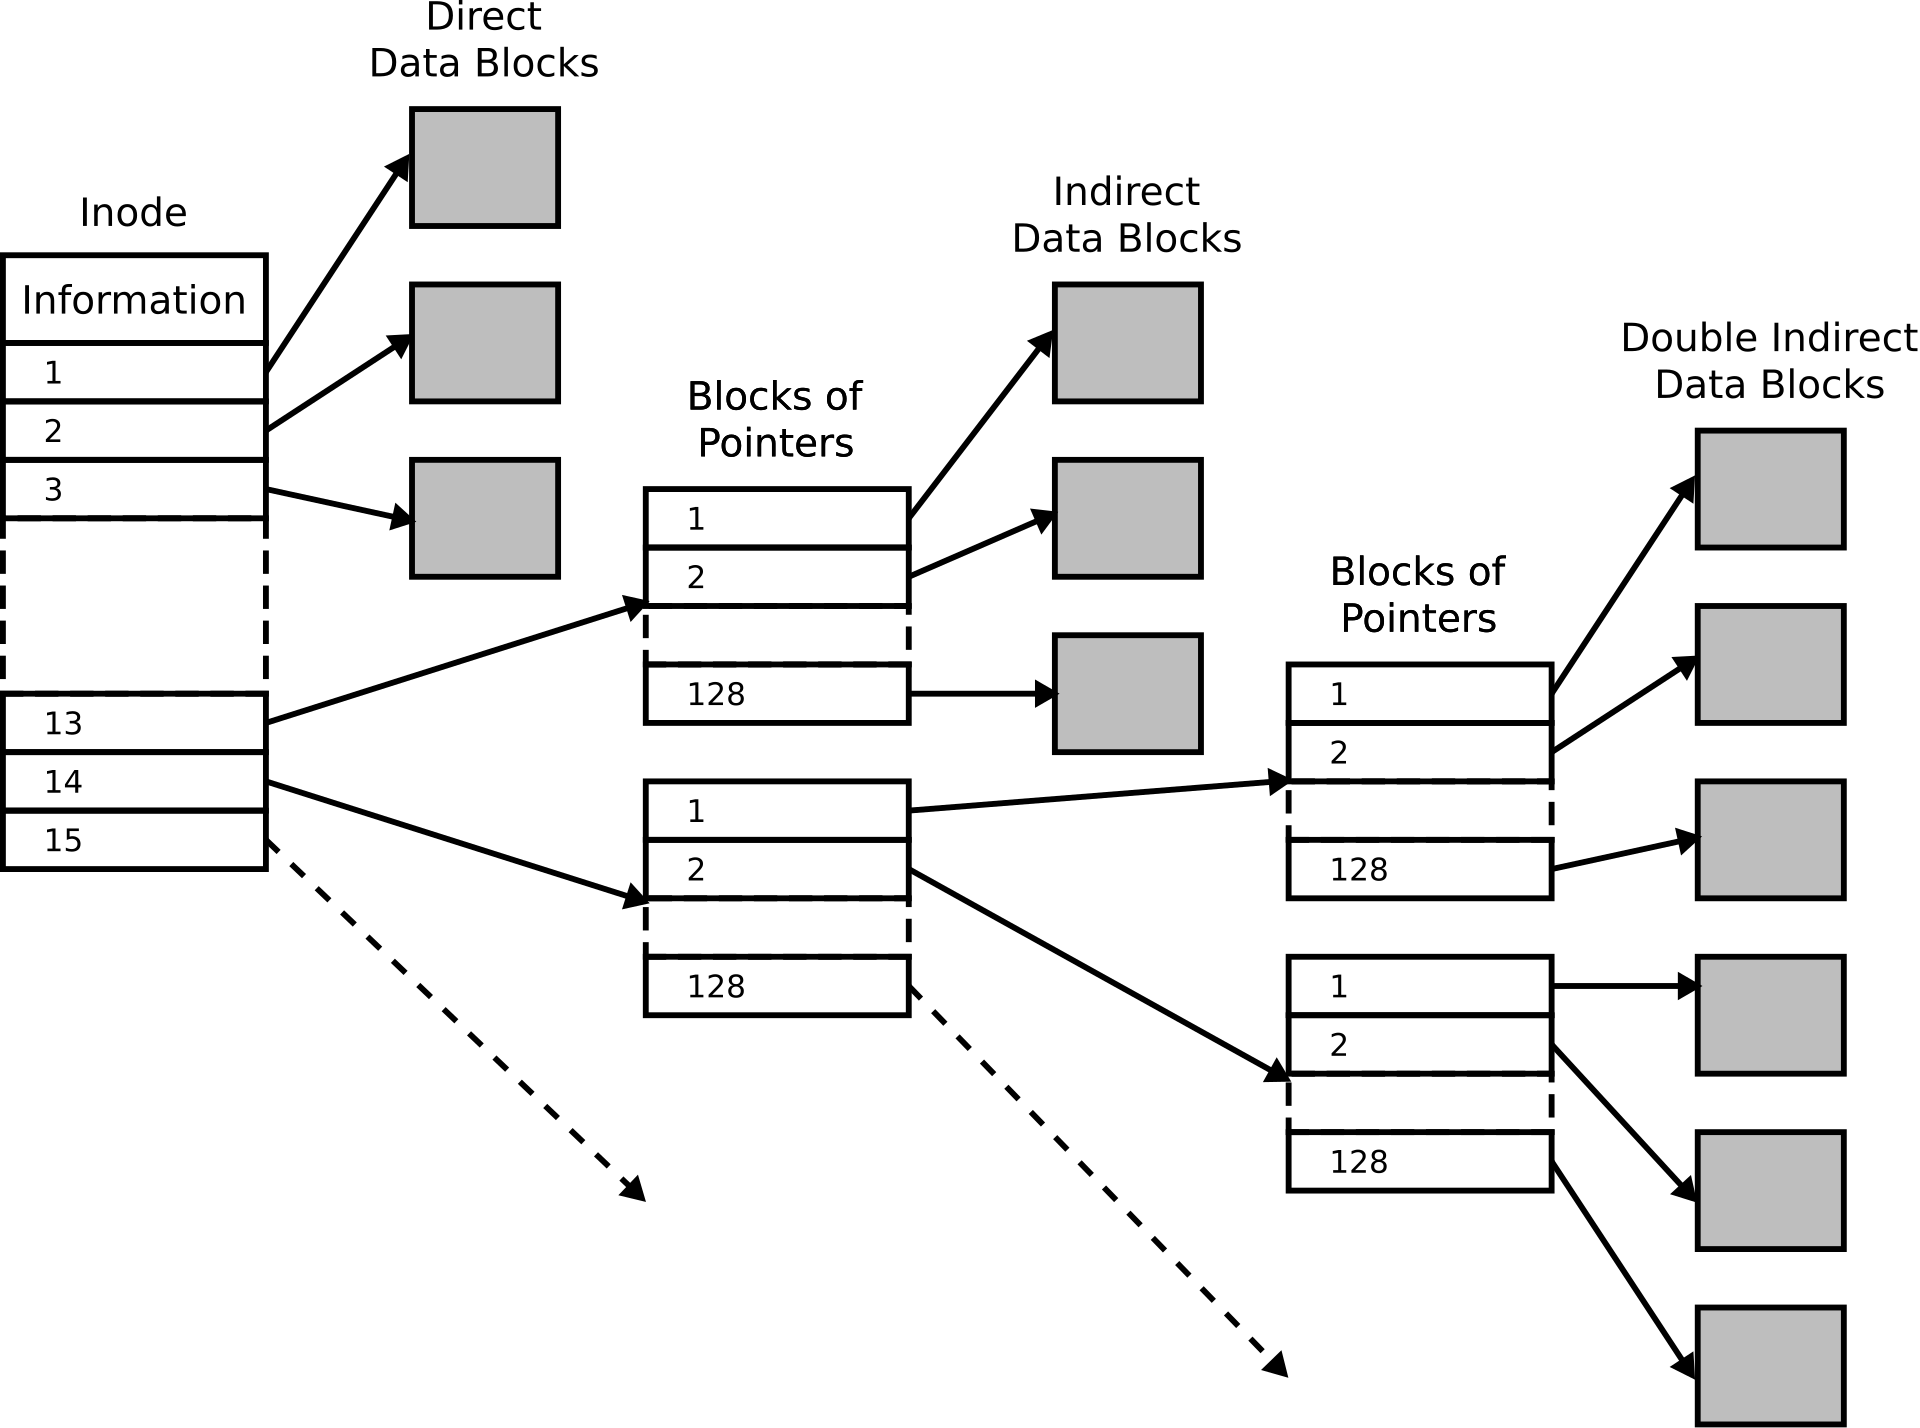
\includegraphics[width=6cm, height=6cm]{address.png}
\caption{Direct and indirect addressing \cite{\href{https://en.wikipedia.org/wiki/Inode_pointer_structure}{C2}}}
\label{fig:3}
\end{figure}
    \item Thus, there is no limit on the size that a file can be in this FS (as long as you have space in hard drive)
\end{itemize}

\section{Miscellaneous discussions}
\begin{itemize}
\item Current language suitable for OS
\begin{itemize}
\item Of the current languages, RUST can be used for writing an OS
\item GO might not be suitable as this has garbage collection, which might not be good for writing an OS
\item There is a concept called pinning, wherein objects are to be statically located in the memory, and if there is garbage collection, then everything must go through this (due to pinning and unpinning), performance is hugely impacted
\item The pinning/unpinning is also the reason why Python is better suited for machine learning algorithms. Since all ML APIs are written in C, C++, programs written in Java have to go through JNI (Java Native Interface) and this does a lot of pinning/unpinning resulting in performance decrease
\end{itemize}
\item Philosophy of UNIX - everything just does one thing, thus the concept of piping in CLI took place
\item This lead to the development of min languages like awk, regular expressions like grep, sed etc.
\item These lead to the development of Perl (which had awk, sed, grep), which in turn lead to the development of Python
\end{itemize}


\end{document}



























